% -*- root: ../../main.tex -*-
\section{File Manager}
\label{sec:file_manager_design}
A seguito di un analisi dei file utilizzati e delle varie risorse caricate da jar e non, sono state individuati tre principali \textbf{categorie} di operazioni.

\hfill \break
Operazioni su:
\begin{enumerate}
    \item \textbf{File generici}
    \item \textbf{File Yaml}
    \item \textbf{Altri dati(musica, sprite, ecc)}
\end{enumerate}

Ogni categoria è gesitita con una classe separata, i file generici sono stati gestiti dal \textbf{FileManager}, i file Yaml con lo \textbf{YamlManager} e gli altri dati con il \textbf{DataManager}.


\begin{figure}[H]
	\centering
	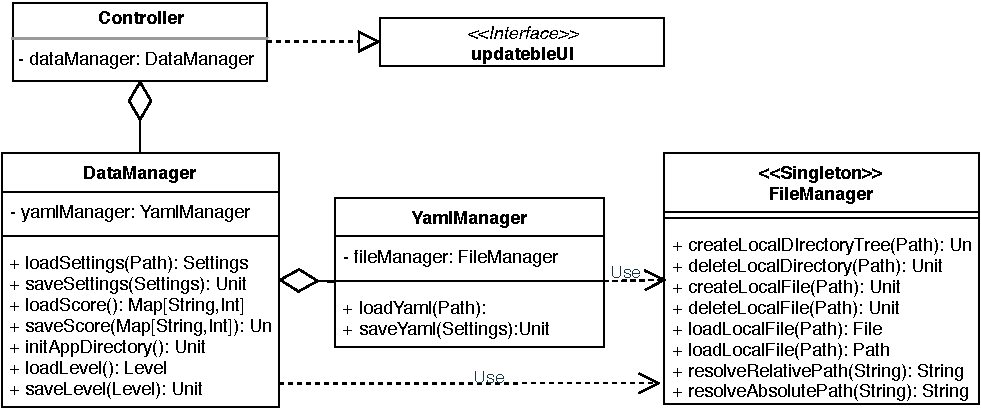
\includegraphics[width=0.90\columnwidth]{drawio/fileManager/fileManager.pdf}
	\caption{Diagramma di classe rappresentante la struttura dei tre.}
	\label{fig:FileManager}
\end{figure}

\begin{itemize}
    \item FileManager: le operazioni di \textbf{base} sui file come il caricamento di una risorsa da jar o da sistema, possono essere effettuate da più punti del programma.
    Un solo FileManager è sufficente per la gestione dei file in tutto l'applicativo, anche per questo è stato reso \textbf{Singleton}.
    Inoltre la divisione dei compiti e l'accesso globale consente di diminuire il rischio di creare \textbf{God class}.
    Per questo il FileManager è un \textbf{Singleton}, 
    \item YamlManager: i file \textbf{Yaml} sono la principale tecnica di \textbf{serializzazione} dei dati utilizzata, in essi vengono salvati livelli, record e dati utente.
    Per questo è stato introdotto un gestore unicamente dedicato ai file Yaml, questo si appoggia sul FileManager per le operazioni di base e ne consente
    scrittura e lettura.
    \item DataManager: consente l'accesso a tutti i dati \textbf{astratti} del programma(livelli, impostazioni, statistiche, ecc).
    Sfrutta lo YamlManager e il FileManager per effettuare le operazioni di caricamento e salvetaggio, è utilizzato dal \textbf{Controller} che lo utilizza per accedere alle varie risorse \textbf{testuali}.
\end{itemize}